\chapter{Evaluation}
\label{sec:evaluation}
% TODO: Segmentation als Metrik
Im Kapitel Evaluation werden die im Kapitel 5 vorgestellten Experimenten evaluiert. Außerdem wird die gewählte Methode ausgewertet und
mit andere Ergebnisse verglichen.

\section{Evaluationsmetrik}
Für das Problem von Image colorization existiert keine relevante Evaluationsmetrik die die Farben von dem Objekten auf einem Bild auswerten kann.
Das während das Training angewendete Cross Entropy Loss ist nicht relevant für die Auswertung der Ergebnisse aus dem Test Datensatz. Aus diesem
Grund wurde die Evaluation der Ergebnisse durch eine Menschliche Auswertung wie bei \cite{zhang2016colorful} und \cite{billaut2018colorunet}
durchgeführt.

\section{Evaluation des Spiel-Datensatzes}
Mit dem Spiel-Datensatz wurde die Funktionsweise der Methode bestätigt. Die von Billaut et al. vorgeschlagene Netzwerkarchitektur für Image
colorization hat beeindruckende Ergebnissen mit wenige Epochen erreicht. 
\\
Die gewählte Methode für das Binning funktionierte und hat ermöglicht die Originale Farben wiederherzustellen. Die Anzahl an 
Bins war für diesen Datensatz nicht relevant da es nur 9 gleich möglichen Farben gab.

\begin{figure}[H]
  \vspace{1cm}
  \centering
  \begin{subfigure}
    \centering
    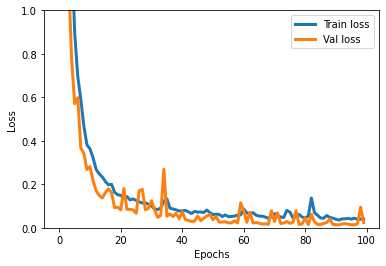
\includegraphics[width=.5\textwidth]{resources/experiments/toy_100_324_0001.png}
  \end{subfigure}
  \caption{Training und Validation Loss Verlauf von dem Spiel-Datensatz}
  \label{image:toy-dataset-loss}
\end{figure}

\section{Evaluation des CIFAR-100 Subsets}
Die Ergebnissen aus dem CIFAR-100 Subset zeigten dass das Model in wenige Epochen viele Merkmale lernen konnte. Ein wichtiger Faktor zu 
erwähnen ist dass die Gewichte des Netzwerks zufällig initialisiert wurden und nicht vortrainiert waren. 
\\
\\
Auf diesem Datensatz wurde die Auswirkung der Bin Anzahl gemessen. Die Auswahl von 36 Bins zeigten im Vergleich zu 324 eine 
Verschlechterung der Farben in der Vorhersage. Dies ist darauf zurückzuführen dass das Model nur 36 mögliche Farben zu Verfügung hat.
Eine Erhöhung der Bins auf 324, ermöglichte das Model eine Auswahl an mehr Farben zu treffen. 
Den Ansatz von \cite{billaut2018colorunet} verwendet nur 32 Bins und erzielt ähnliche Ergebnisse wie die Methode dieser Arbeit mit 324 Bins.
Dies wurde erreicht in dem die Pixeln von jedem Trainingsbild vor dem Training in Bins klassifiziert wurde und daraus nur die am meisten
Vorkommende 32 Bins ausgewählt wurden. Pixeln die nicht in den gewählten 32 Bins klassifiziert werden konnten, wurden in das nächstliegende Bin
zugeordnet.
\\
Der Methode mit einem MSE Loss ermöglicht eine um ein vielfaches größere Auswahl an Farben für die Vorhersage. Bei dieser Methode tretten 
die im Kapitel \ref{subsection:verwandte-arbeiten} erwähnten Schwierigkeiten, wobei in dem Fall von diesem Datensatz die kaum zu erkennen waren.
Da die Klassifikationsmethode bessere Ergebnissen geliefert hat, wurden alle Experimenten des Landscape Datensatzes mit dieser Methode durchgeführt.
\\
\\
Der Verlauf von dem Training und Validation Loss deutete bei diesem Datensatz zu overfitting, was bei der Große des Datensatzes vorkommen kann.
Wie bei \ref{section:cifar-experimente} beschrieben würde das U-net und die Hyperparameter angepasst um dieses zu verhindern.

\begin{figure}[H]
  \centering
  \vspace{1cm}
  \begin{subfigure}
    \centering
    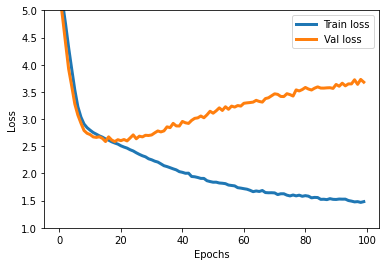
\includegraphics[width=.48\textwidth]{resources/experiments/cifar_100_324_0001.png}
  \end{subfigure}
  \begin{subfigure}
    \centering
    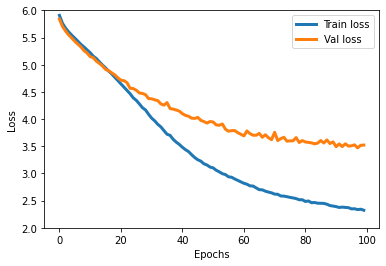
\includegraphics[width=.48\textwidth]{resources/experiments/cifar_100_324_00001.png}
  \end{subfigure}

  \caption{Overfitting auf dem CIFAR-100 Subset. \textbf{Links}: 100 Epochen mit Adam, ReLU und eine Lernrate von 0.001. \textbf{Rechts}:
  100 Epochen mit Adam, ReLU und eine Lernrate von 0.0001.}
  \label{image:gute-ergebnisse-cifar}
\end{figure}

Eine Anpassung der Lernrate führte nur zu einem langsameres Training. Eine Reduktion der lernbare Parameter von 135684 auf 35748 zeigte 
eine deutliche Verbesserung der Performance des Models und reduzierte das Overfitting.

\begin{figure}[H]
  \centering
  \vspace{1cm}
  \begin{subfigure}
    \centering
    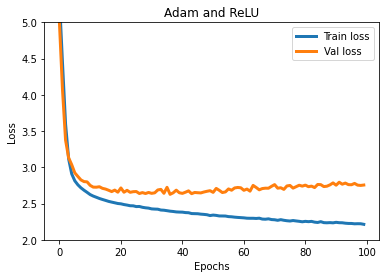
\includegraphics[width=.48\textwidth]{resources/experiments/cifar-adam-relu.png}
  \end{subfigure}
  \begin{subfigure}
    \centering
    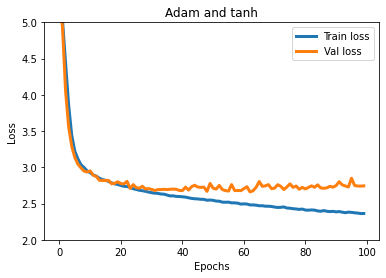
\includegraphics[width=.48\textwidth]{resources/experiments/cifar-adam-tanh-100.png}
  \end{subfigure}

  \caption{Loss Verlauf mit eine reduzierte Anzahl an Parameter und verschiedene Aktivierungsfunktionen. 
  \textbf{Links}: 100 Epochen mit Adam, ReLU und eine Lernrate von 0.001. \textbf{Rechts}: 100 Epochen mit Adam, Tanh und eine Lernrate von 0.001.}
  \label{image:gute-ergebnisse-cifar}
\end{figure}

Der Grund für das Overfitting ist in diesem Fall zu der Große des Subsets zurückzuführen. Um das zu prüfen wurde das Model auf das komplette CIFAR-100
Datensatz für 150 Epochen trainiert, was einen guten Loss Verlauf zeigte. Auf der anderen Seite, hat das Model nichts relevantes gelernt und 
konnte kein Bild richtig einfärben, was bei der Anzahl der Klassen und die Anzahl der Epochen normal ist.

\section{Evaluation des Landscape Datensatzes}
% Beispiel einer Tabelle:
% \begin{longtable}{|c|c|c|c|}
% 	\hline
% 	\multicolumn{1}{|c}{\textbf{Spalte 1}} &
% 	\multicolumn{1}{|c}{\textbf{Spalte 2}} &
% 	\multicolumn{1}{|c|}{\textbf{Spalte 3}} \\
% 	\hline
% 	\endfirsthead
	
% 	\multicolumn{3}{c}{Beschreibung}\\ \hline
% 	\multicolumn{1}{|c}{\textbf{Spalte 1}} &
% 	\multicolumn{1}{|c}{\textbf{Spalte 2}} &
% 	\multicolumn{1}{|c|}{\textbf{Spalte 3}} \\
% 	\hline
% 	\endhead
	
% 	\multicolumn{2}{c}{Fortsetzugn auf der nächsten Seite}
% 	\endfoot
	
% 	\caption{Beschreibung}
% 	\label{tab:example}
% 	\endlastfoot
	
% 	TODO & TODO & TODO \\ \hline
% 	TODO & TODO & TODO  \\ \hline
% \end{longtable}

% \section{Beispiel Unterkapitel}
% TODO